\documentclass{article}
\setlength{\parindent}{0ex}
\setlength{\parskip}{1em}
\usepackage[utf8]{inputenc} 
\usepackage{amsfonts}
\usepackage{amssymb}
\usepackage{amsmath}
\usepackage{amstext}
\usepackage{fancybox}
\usepackage{tikz}
\usepackage{tkz-euclide}
\usepackage{gensymb}
\usepackage{graphicx}
\usepackage{verbatim}
\usepackage{qtree}
\usepackage{scrextend}
\usepackage{multirow}
\usepackage{float}

\tikzset{main node/.style={circle,fill=blue!20,draw,minimum size=1cm,inner sep=0pt},
}

%Kodestyling \begin{lstlisting}
\usepackage{color}
\usepackage{listings}
\lstset{ %
language=C++,                % choose the language of the code
%basicstyle=\footnotesize,       % the size of the fonts that are used for the code
basicstyle=\ttfamily,
%numbers=left,                   % where to put the line-numbers
numberstyle=\footnotesize,      % the size of the fonts that are used for the line-numbers
stepnumber=1,                   % the step between two line-numbers. If it is 1 each line will be numbered
numbersep=5pt,                  % how far the line-numbers are from the code
backgroundcolor=\color{white},  % choose the background color. You must add \usepackage{color}
showspaces=false,               % show spaces adding particular underscores
showstringspaces=false,         % underline spaces within strings
showtabs=false,                 % show tabs within strings adding particular underscores
%frame=single,           % adds a frame around the code
tabsize=2,          % sets default tabsize to 2 spaces
captionpos=b,           % sets the caption-position to bottom
breaklines=true,        % sets automatic line breaking
breakatwhitespace=false,    % sets if automatic breaks should only happen at whitespace
escapeinside={\%*}{*)},          % if you want to add a comment within your code
mathescape
}

\usepackage{mathtools}
\DeclarePairedDelimiter\ceil{\lceil}{\rceil}
\DeclarePairedDelimiter\floor{\lfloor}{\rfloor}


\def\meta#1{\mbox{$\langle\hbox{#1}\rangle$}}
\def\macrowitharg#1#2{{\tt\string#1\bra\meta{#2}\ket}}

{\escapechar-1 \xdef\bra{\string\{}\xdef\ket{\string\}}}

\def\intro#1{{#1}{\cal I}}
\def\elim#1{{#1}{\cal E}}

\showboxbreadth 999
\showboxdepth 999
\tracingoutput 1


\let\imp\to
\def\elim#1{{{#1}{\cal E}}}
\def\intro#1{{{#1}{\cal I}}}
\def\lt{<}
\def\eqdef{=}
\def\eps{\mathrel{\epsilon}}
\def\biimplies{\leftrightarrow}
\def\flt#1{\mathrel{{#1}^\flat}}
\def\setof#1{{\left\{{#1}\right\}}}
\let\implies\to
\def\KK{{\mathsf K}}
\let\squashmuskip\relax

\graphicspath{ {images/} }
\usetikzlibrary{arrows}
\tikzset{
  leaf_/.style = {shape=rectangle,draw, align=center},
  node_/.style     = {shape=circle,draw,align=center}
}
\author{Rune Kok Nielsen (qkd362), Andreas Holm (jnh508)}
\title{Afløsningsopgave i fagområdet Modellering og Analyse af Data}
\DeclareMathOperator{\Ran}{Ran}
\DeclareMathOperator{\Dom}{Dom}
\begin{document}

\maketitle

\section{Klassificering}
Formålet med klassificering er at putte datapunkter bestående af et antal egenskaber i passende kategorier fra en prædifineret mængde af diskrete, beskrivende kategorier, disse datapunkter er også kendt som tupler bestående af $(x,y)$, hvor $x$ er de givet egenskaber, og $y$ er dens kategori. Klassificering består i definitionen af at finde en passende klassificeringsmodel, hvilket er en funktion $f$ der tager et datapunkt $x$ og returnerer den tilhørende kategori $y$.

Der findes adskillige teknikker til at bestemme en klassificeringsmodel. En sådan teknik beskriver en læringsalgoritme, der på basis af et træningssæt (et sæt af datapunkter med kendte kategorier) udleder en (evt. suboptimal) model.

Det er sjældent muligt at klassificere ethvert givent punkt korrekt ud fra de tilgængelige egenskaber, og vi har derfor brug for en måde at afgøre nøjagtigheden af den resulterende model. Denne nøjagtighed estimeres ved at klassificere et testsæt med modellen, og se på hvor stor en andel af datapunkterne der har fået den rigtige kategori. For at vise modellens nøjagtighed kan man beregne dens \textit{accuracy}, hvilket fortæller hvor præcis den er, eller man kan beregne dens \textit{error rate}, hvilke er det modsatte af \textit{accuracy} dvs. hvor mange forkerte punkter modellen har produceret. For at beregne disse målenheder bruger vi en \textit{confusion matrix}. I table 1 ses en \textit{confusion matrix}, det ses i kolonnerne hvad modellen har tildelt klassen, og i rækkerne ses hvad dens rigtige klasser er. \\

\begin{table}[H]
\begin{center}
\begin{tabular}{cc|c|c|c|c|}
    & \multicolumn{5}{c}{Predicted Class} \\
    \cline{3-6}
     & & Class = 0 & Class = 1 & .. & Class = n \\
    \cline{2-6}
    \multicolumn{1}{c|}{\multirow{4}{*}{Actual Class}} & Class = 0 & $f_{00}$ & $f_{01}$ & .. & $f_{0n}$ \\
    \cline{2-6}
    \multicolumn{1}{c|}{} & Class = 1 & $f_{10}$ & $f_{11}$ & .. & $f_{1n}$ \\
    \cline{2-6}
    \multicolumn{1}{c|}{} & .. & .. & .. & .. & .. \\
    \cline{2-6}
    \multicolumn{1}{c|}{} & Class = m & $f_{m0}$ & $f_{m1}$ & .. & $f_{mn}$ \\
    \cline{2-6}
\end{tabular}
\caption{\textit{Confusion matrix}}
\end{center}
\end{table}

For at beregne vores \textit{accuracy} og \textit{error rate} bruger vi vores tabel, og har således en formel for hver målenhed, som kan ses nedenfor. \\

\begin{align*}
Accuracy &= \frac{Antallet \ af \ korrekte \ forudsigelser}{Det \ totale \ antal \ forudsigelser} \\
         &= \frac{f_{00} + f_{11} + f_{mn}}{f_{00} + f_{01} + f_{0n} + f_{10} + f_{11} + f_{1m} + f_{m0} + f_{m1} + f_{mn}}
\end{align*}

\begin{align*}
Error \ rate &= \frac{Antallet \ af \ forkerte \ forudsigelser}{Det \ totale \ antal \ forudsigelser} \\
           &= \frac{f_{01} + f_{0n} + f_{10} + f_{1n} + f_{m0} + f_{m1}}{f_{00} + f_{01} + f_{0n} + f_{10} + f_{11} + f_{1m} + f_{m0} + f_{m1} + f_{mn}}
\end{align*}

Her gælder det at jo højere \textit{accuracy} desto bedre, og det modsatte gælder for \textit{error rate}. \\

\subsection{Beslutningstræer (Decision trees)}
Et eksempel på en klassificeringsteknik er gennem brug af beslutningstræer. Et beslutningstræ består af knuder og blade samt en rodknude. Et datapunkt kan da klassificeres ved at traversere træet startende i roden.

Hver knude består af et spørgsmål, som har en definitiv mængde svar, der kan besvares ud fra egenskaberne i et givent datapunkt. Ud fra svaret (altså datapunktets egenskaber) peger knuden videre til en ny knude eller et blad. Et blad repræsenterer den endelige kategori. I eksemplet i figur 1, kan der ses et eksempel på hvordan et \textit{decision tree} fungere, i dette eksempel antager vi, vi har fået en mængde, som indeholder enten biler, fly eller både, vi starter med at spørge om det givet datapunkt har hjul, hvis nej må det være en båd, hvis ja kan det enten være en bil eller et fly, og derfor spørger vi igen, denne gang om det givet datapunkt har vinger, hvis ja er det et fly, og hvis nej må det være en bil, på denne måde har vi sikret os at vores datapunkt er kommet i den rigtige kategori.

\begin{figure}[H]
\begin{center}
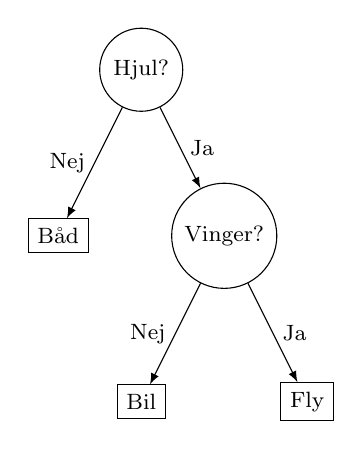
\begin{tikzpicture}
  [
    grow                    = down,
    sibling distance        = 6em,
    level distance          = 6em,
    edge from parent/.style = {draw, -latex},
    every node/.style       = {font=\footnotesize}
  ]
  \node [node_] {Hjul?}
    child { node [leaf_] {Båd}
      edge from parent node [left] {Nej} }
    child { node [node_] {Vinger?}
      child { node [leaf_] {Bil}
              edge from parent node [left]{Nej} }       
      child { node [leaf_] {Fly}
              edge from parent node [right]{Ja} }
              edge from parent node [right] {Ja} };
\end{tikzpicture}
\end{center}
\caption{\textit{Decision tree} eksempel}
\end{figure}

Et (muligvis suboptimalt) beslutningstræ kan bl.a. konstrueres fra et træningssæt med Hunts algoritme. Algoritmen starter med en mængde af alle datapunkter i træningssættet. Hvis alle punkter i mængden har samme kategori bliver denne mængde et blad i træet. Ellers stilles et spørgsmål om punkterne i mængden, og disse punkter uddeles samles i delmængder ud fra, hvordan de besvarer spørgsmålet. Spørgsmålet bliver en knude i træet, som peger på de nye delmængder, og algoritmen køres rekursivt på delmængderne.



\end{document}